%!TEX root = ../../../thesis.tex

The amount of energy lost in a mechanical water meter has been estimated, as has the fraction of that energy which can be harnessed.
Now, the amount of energy required to operate an electronic water meter is estimated.
This estimation will show how far the streaming cells made earlier are away from being a viable harvesting option.

\section{Microcontrollers}

  Central to the operation of an electronics water meter is the microcontroller (MCU).
  The primary function of the microcontroller is to read and log the amount of water consumed by the meter.
  It will also decide when to transmit that data and monitor its own energy usage.
  It is therefore a key component of the electronic meter and is expected to consume the majority of its energy.

  In this chapter I compare power consumption and operational efficiencies of six low power MCUs deemed suitable for use in a water meter.
  The microprocessors to be investigated are low power, general purpose, 8-bit processors from Microchip, Atmel and Freescale.
  The measured functions are analogue-to-digital conversion, non-volatile memory writes, processing, and clocking.
  These functions are believed to be important for the intended application.


  \subsection{Selection of appropriate controllers}

    \begin{sidewaystable}
      \begin{centering}
        \begin{tabular}{|l|l|l|l|l|l|l|l|}
        \cline{2-8}
        \multicolumn{1}{l|}{} & PIC16F1827  & PIC16F887  & PIC16F688  & PIC12F675  & ATtiny25V  & ATtiny13V  & MC9S08QG8 \tabularnewline
        \hline
        Vdd (min)  & 1.8  & 2.0  & 2.0V  & 2.0  & 1.8  & 1.8  & 1.8 \tabularnewline
        Vdd (max)  & 5.5  & 5.5  & 5.5V  & 5.5  & 5.5  & 5.5  & 3.6 \tabularnewline
        I (sleep)  & 30nA  & 50nA  & 50nA  & 1nA  & 100nA & <100nA & 450nA\tabularnewline
        CLOCK (min)  & 31kHz  & 31kHz & 31kHz & 31kHz & 16kHz & 16kHz & 1MHz \tabularnewline
        CLOCK (max)  & 32MHz  & 8MHz  & 8MHz  & 4MHz  & 16MHz & 9MHz  & 10MHz\tabularnewline
        EEPROM  & 256B  & 256B  & 256B  & 128B  & 128B  & 64B  & \dag{}\tabularnewline
        Serial  & USI  & USI  & USI  & --  & USI  & --  & USI \tabularnewline
        USART  & UART  & UART  & UART  & --  & --  & --  & -- \tabularnewline
        ADC  & 10bit  & 10bit & 10it  & 10bit & 10bit & 10bit & 10bit\tabularnewline
        \hline
        \end{tabular}
      \end{centering}

      \begin{centering}
      \dag Has 8,192 bytes of software programmable flash (16 pages of 512 bytes each).
      \end{centering}

      \begin{centering}
      \ddag Has 256 bytes of software programmable flash (4 pages of 64 bytes each).
      \end{centering}

      \caption{\label{tab:MCUfeaturecomparison} Feature comparison of selected MCUs.}
    \end{sidewaystable}

    The following processors were chosen the three chosen manufacturers.
    \begin{itemize}
    \item Microchip PIC16F1827
    \item Microchip PIC16F688
    \item Microchip PIC12F675
    \item Atmel ATtiny25V
    \item Atmel ATtiny13V
    \item Freescale MC9S08QG8
    \end{itemize}
    A basic feature comparison of the MCU selection is shown in table \ref{tab:MCUfeaturecomparison}.





% \section{Power consumption}

% Each of the MCUs were programmed to carry out various tasks which
% were performed over their specified range of operating voltages and
% operating frequencies. While the chips where carrying out these tasks
% their power consumption was measured by an Agilent E5270B Precision
% Mainframe via a PC and a Tektronix MSO 4054 Oscilloscope for timing
% purposes. Details on how each of the tests where carried out, as well
% as raw data, can be found in appendix %\ref{Appendix:Measurements} .


  \subsection{Power consumption benchmarks}

    Testing the power consumption of low-power microprocessors requires a few taking precautions.
    The chips must be configured to ensure that do not consume more power than is necessary.
    Where possible, the chips were configured to have each of their pins set to outputs, which were held high while being tied to Vdd via 10k$\Omega$ resistors.
    All chips had their peripherals disabled (where appropriate) including any watchdog timers and brownout detection circuitry.
    To allow more accurate sleep current measurements, the chips were placed in a chip carrier with 10k$\Omega$ resistors soldered between the pins (except ground and Vdd) and Vdd.
    They chip and carrier was then washed in isopropyl alcohol and dried before being suspended by connections to the measurement device.
    This was done to reduce any current leakage between pins due to fingerprints or dirt.
    Measurements were carried out using the Agilent E5270B Precision Measurement Mainframe.
    This device has been used for most other measurement situations throughout this thesis for its high impedance inputs and measurement accuracy.


    \subsubsection*{Sleeping}


      \begin{figure}
        \centering
        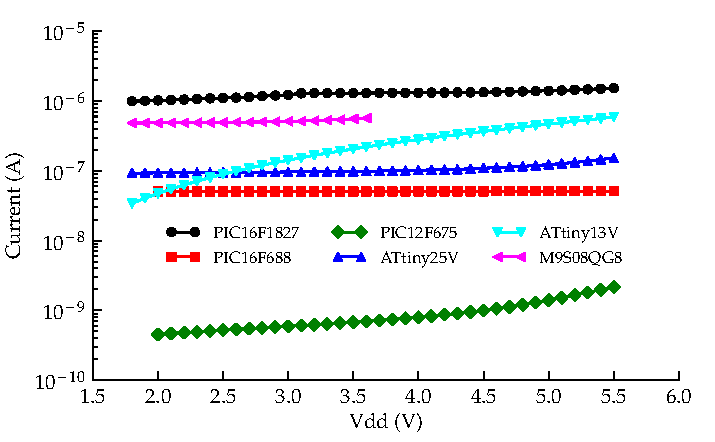
\includegraphics{content/pt1/03-EnergyRequirements/graphics/Graph_All_Sleeping_Current}
        \caption{\label{fig:All_Sleep_Current}Current consumed by investigated MCUs while in sleep mode.}
      \end{figure}

      A microprocessor in sleep mode is essentially powered off, the difference being that volatile data is preserved.
      In order to consume as little power as possible an MCU should spend as much time in sleep mode as possible.
      Therefore, power consumption in sleep states will determine a large part of the chips overall power consumption.

      \cref{fig:All_Sleep_Current} shows the amount of current consumed by each MCUs while in their deepest sleep states.
      Surprisingly, the PIC16F1827 consumes the most current in this state, almost one thousand times more than the specified sleep current of \SI{30}{\nano\ampere}\cite{PIC16F1827}.
      The Freescale MC9S08QG8 consumed energy at an average of 11\% higher than specified \cite{MC9S08QG8}.
      Both the Atmel ATtiny13V and ATtiny25V fell within their specification, \cite{AtmelATtiny13,AtmelATtiny25} respectively.
      The Microchip PIC12F675 fell within specification\cite{PIC12F675} and was clearly ahead in terms of minimum current draw during sleep.

      There appears to be a trade-off between the two Atmel processors in the way of minimum power consumption and minimum response to Vdd.
      The ATtiny13V required approximately 2.7 times less power than the ATtiny25V at 1.8V, but above 2.5V the ATtiny25V is more draws less current.

      As the PIC16F1827 was so far off its specified value, measurements were repeated numerous times using code written in both assembler and HI-TECH C.
      A total of five different processors were tried, all giving the same result.
      All steps outlined in the PIC16F1827's datasheet to reduce power consumption had been followed.


    \subsubsection*{Disclaimer on processing}


      Measuring the amount of power it takes to process information is not a simple task.
      The way each chip carries out processing operations internally can be quite different from one another, even though they
      all produce the same result.

      \begin{table}
        \centering
        \begin{tabular}{|c|c|}
          \cline{2-2}
          \multicolumn{1}{c|}{} & Instructions\tabularnewline
          \hline
          PIC16F1827 & 53\tabularnewline
          \hline
          PIC16F688 & 35\tabularnewline
          \hline
          PIC12F675 & 35\tabularnewline
          \hline
          ATtiny25V & 120\tabularnewline
          \hline
          ATtiny13V & 120\tabularnewline
          \hline
          MC9S08QG8 & 145\tabularnewline
          \hline
        \end{tabular}
        \caption{\label{tab:Number-of-instructions}Instruction set size for each tested MCU.}
      \end{table}


      \begin{algorithm}[H]
        \begin{lstlisting}
        if (danger >= 5) flight();
        else flee();
        \end{lstlisting}
        \caption{\label{alg:Simple-C-code-representation}Simple C-code representation of a branch instruction.}
      \end{algorithm}


      Algorithm \ref{alg:Simple-C-code-representation} shows a simplified programme.
      To determine whether the programme's outcome, the processor must first evaluate whether `danger' is greater than or equal to five.
      Then it will either branch to the function `flight' or continue on to execute the function `flee'.

      \begin{algorithm}
        \begin{lstlisting}
        load 5 into register 001
        load danger into register 002
        branch-if-greater-or-equal 001 002 flee_call
        call-subroutine fight
        jump-to continue
        [flee_call]
        call-subroutine flee
        [continue]
        \end{lstlisting}
        \caption{\label{alg:Psudo-machine-code1}Psudo machine-code representation
        of a branch instruction.}
      \end{algorithm}

      \begin{algorithm}
        \begin{lstlisting}
        load danger into register 001
        subtract-from-register 001 5
        branch-if-minus 001 fight_call
        call-subroutine flee
        jump-to continue
        [fight_call]
        call-subroutine fight
        [continue]
        \end{lstlisting}
        \caption{\label{alg:Psudo-machine-code2}Psudo machine-code representation of an alternative branch instruction.}
      \end{algorithm}


      Algorithms \ref{alg:Psudo-machine-code1} and \ref{alg:Psudo-machine-code2} demonstrate two different ways of implementing \ref{alg:Simple-C-code-representation} using pseudo machine-code.
      The decision of which is best is made by the compiler, which should take the instructional efficiency of the specific MCU into account.
      This is an overly simplistic example, but it illustrates that there are multiple paths leading to the same result.
      Importantly, not all of those paths require the same amount of effort on the processors behalf.
      This means that the compiler's ability to optimise code efficiently plays a role in determining the overall performance of the chip.
      This also means that the programmer shouldn't need to worry too much about instructional efficiency as the compiler should transform C-code into machine code that best suits the target MCU.

      Another factor in processing efficiency comes down to the number of different instructions it can do.
      This list of instructions a processor is capable of is its instruction set.
      Most 8-bit MCUs are based on reduced instruction set computing (RISC) architecture, as opposed to complex instruction set computing (CISC).
      When compared CISC based CPU, a RISC based chip is simpler and therefore usually cheaper to produce.
      However, ``Instruction traces from CISC machines consistently show that few of the available instructions are used in most computing environments''\cite{ComputerArch}.
      This means that many of the extended operations in in CISC designs are underutilised.
      Processors with smaller instruction sets are capable of achieving the more complex operations by chaining multiple instructions together.
      This means that processors with smaller instruction sets will take longer to achieve certain instructions.
      Finally, the frequency of a microprocessor isn't necessarily the frequency at which it performs operations, although sometimes it is.
      For instance, the Atmel and Freescale microprocessors perform one instruction per clock cycle, whereas the Microchip processors perform one instruction every four clock cycles.


    \subsubsection*{Power consumed while processing}

      \begin{figure}
        \centering
        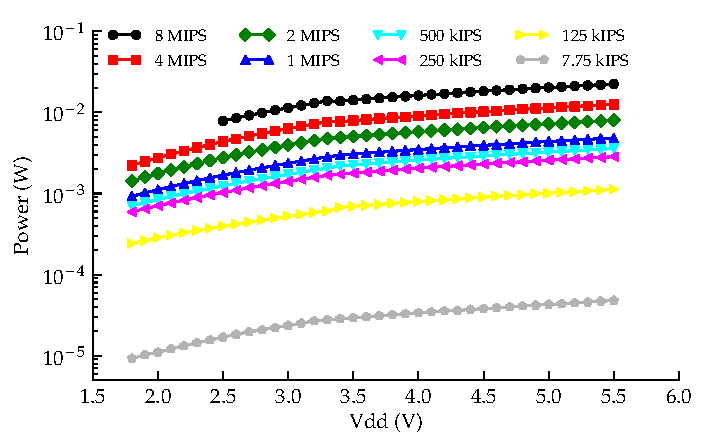
\includegraphics{content/pt1/03-EnergyRequirements/graphics/Graph_PIC16F1827_Clock_Power}
        \caption{\label{graph:CLK_POWER_16F1827}Power consumed by the PIC16F1827 while processing}
      \end{figure}

      \begin{figure}
        \centering
        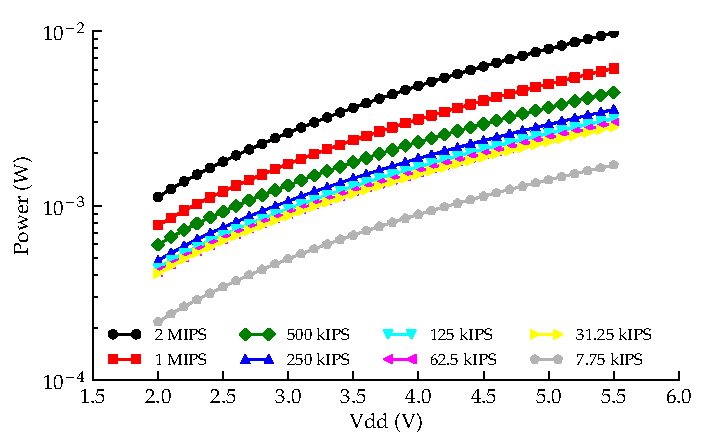
\includegraphics{content/pt1/03-EnergyRequirements/graphics/Graph_PIC16F688_Clock_Power}
        \caption{\label{graph:CLK_POWER_16F688}Power consumed by the PIC16F688 while processing}
      \end{figure}

      \begin{figure}
      \centering
        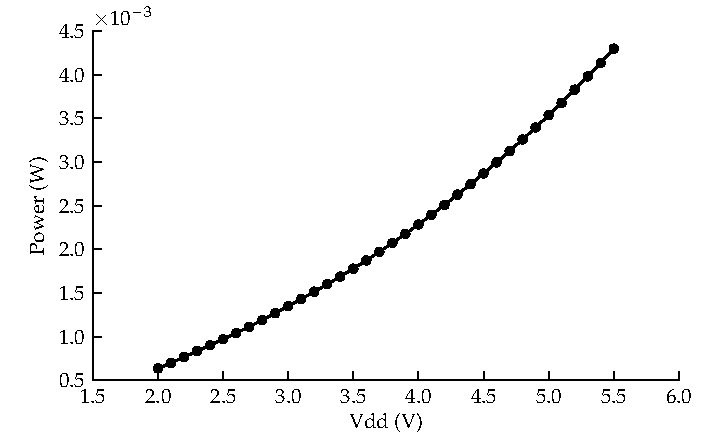
\includegraphics{content/pt1/03-EnergyRequirements/graphics/Graph_PIC12F675_Clock_Power}
        \caption{\label{graph:CLK_POWER_12F675-1}Power consumed by the PIC12F675 while processing}
      \end{figure}

      \begin{figure}
      \centering
        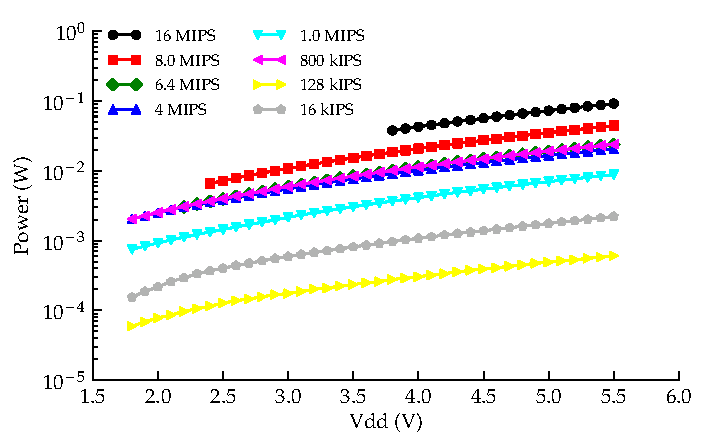
\includegraphics{content/pt1/03-EnergyRequirements/graphics/Graph_ATtiny25V_Clock_Power}
        \caption{\label{graph:CLK_POWER_ATtiny25V}Power consumed by the ATtiny25V while processing}
      \end{figure}

      \begin{figure}
        \centering
        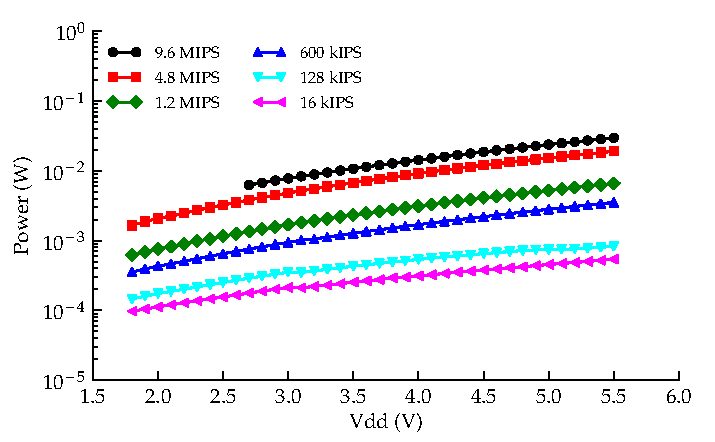
\includegraphics{content/pt1/03-EnergyRequirements/graphics/Graph_ATtiny13V_Clock_Power}
        \caption{\label{graph:CLK_POWER_ATtiny13V}Power consumed by the ATtiny13V while processing}
      \end{figure}

      \begin{figure}
        \centering
        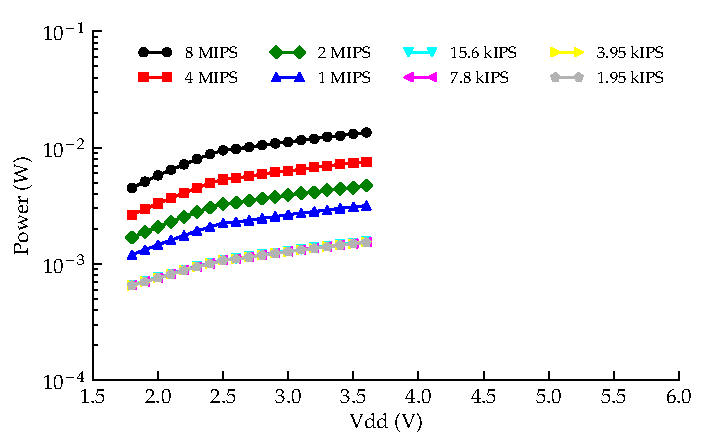
\includegraphics{content/pt1/03-EnergyRequirements/graphics/Graph_MC9S08QG8_Clock_Power}
        \caption{\label{graph:CLK_POWER_MC9S08QG8}Power consumed by the MC9S08QG8 while processing}
      \end{figure}

      Results in this section are expressed in terms of instructions per second (IPS).
      The Microchip PIC16F1827 displayed the lowest energy usage with \SI{10}{\micro\ampere} while clocking \SI{7.75}{\kilo IPS} (as shown in \cref{graph:CLK_POWER_16F1827}).
      Microchip MCUs complete one instruction every four clock cycles, so the \SI{7.75}{\kilo IPS} actually corresponds to a standard clock frequency of \SI{31}{\kilo\hertz}.

      \Cref{graph:CLK_POWER_16F688} shows the PIC16F688 consumes less power than the PIC16F1827 while at low voltages for the same instruction rates (except at 7.75kIPS).
      There appears to be a flatter response in power consumption with respect to Vdd in the PIC16F1827.
      Again, this appears to be a similar trade-off to that made earlier in \cref{fig:All_Sleep_Current} with the Atmel chips.

      The PIC12F675 (\cref{graph:CLK_POWER_16F688}) used the same at the PIC16F688 (\cref{graph:CLK_POWER_16F688}) for its \SI{1}{\mega IPS} trace.
      \Cref{graph:CLK_POWER_ATtiny25V,graph:CLK_POWER_ATtiny13V} show both Atmel MCUs having similar requirements.
      The MC9S08QG8, although being able to clock the slowest, performed very poorly at low frequencies.
      At \SI{1.95}{\kilo IPS} it consumed approximately the same amount of power as the Microchip MCUs operating at \SI{1}{\mega IPS}.

    \subsubsection*{Joules of energy consumed per instruction cycle\label{sub:Joules-of-energy}}

A convenient, and more insightful way to interpret the previous processing
power consumption graphs is to calculate the energy spent per instruction
performed. The energy cost of an instruction cycle can be calculated
using equation \ref{eq:JPI calculation}.

\begin{equation}
J_{i}=\frac{I\times Vdd}{f_{i}}\label{eq:JPI calculation}
\end{equation}
where $J_{i}$ is the number of joules consumed per instruction, $I$
is the current draw, $Vdd$ is the input voltage and $f_{i}$ is the
instruction frequency.

Figure \ref{fig:Per-instruction-cycle} compares the most energy efficient
operating conditions of each of the tested chips. What is most interesting
about this graph is amount of overlap between each of the chips. Also,
these greater efficiencies occur at high operating frequencies. A
simple rule of thumb for selecting the most power efficient operating
frequency based on these results is to choose the highest frequency
where the MCU can operate over its full input voltage (Vdd) range.
For comparison, figure \ref{fig:Per-instruction-ATtiny13V} shows
the trade-off made when selecting a higher frequency, which is typical
across the range of MCUs tested.

\begin{figure}
\begin{centering}
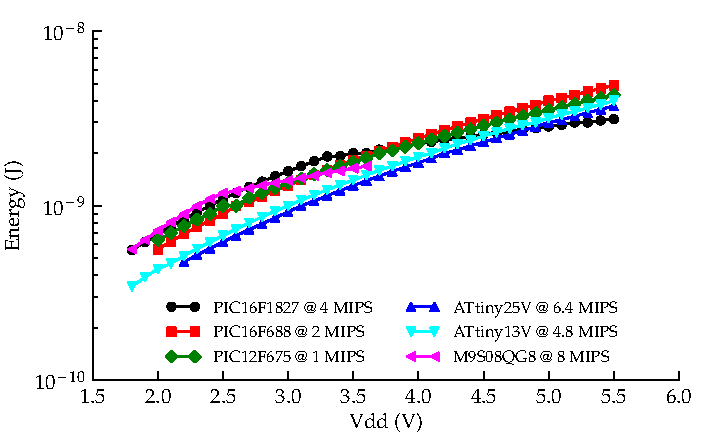
\includegraphics{content/pt1/03-EnergyRequirements/graphics/Graph_All_Clock_JPI}
\par\end{centering}

\protect\caption{\label{fig:Per-instruction-cycle}Per instruction cycle energy consumption
comparison}
\end{figure}
\begin{figure}
\begin{centering}
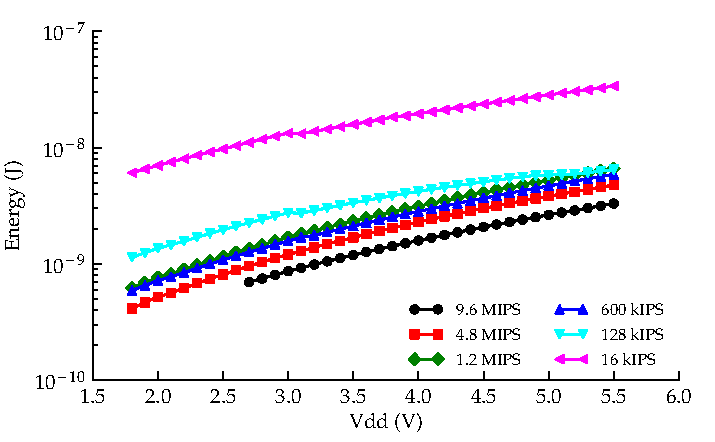
\includegraphics{content/pt1/03-EnergyRequirements/graphics/Graph_ATtiny13V_Clock_JPI}
\par\end{centering}

\protect\caption{\label{fig:Per-instruction-ATtiny13V}Per instruction cycle energy
consumption of the ATtiny13V}
\end{figure}



\subsubsection*{Performance benchmark}

In section \ref{sub:Joules-of-energy} I presented a graph showing
the amount of energy consumed per instruction cycle for each MCU under
ideal operating conditions. But, as discussed in section \ref{sub:Behind-the-scenes},
not all instructions take one instruction cycle to complete. Also,
some MCUs have extra instructions that are designed to help speed-up
code execution by combining commonly used pairs of instructions. This
section will look at how many instruction cycles each MCU takes to
complete a benchmarking function. Which will allow a more accurate
representation of execution efficiency to be made.

For the benchmarking function I wanted something that would consume
a large number of instructions cycles, be well suited to an 8-bit
microcontroller (i.g. no complex maths functions and small memory
footprint) and have a well defined end point. For this I chose a linear
feedback shift register based pseudo-random number generator (as shown
in \ref{alg:Benchmarking-algorithm}), for which the code was sourced
from \cite{LinearFeedbackRegister}.

In short, this function starts with a 16-bit number and runs it through
the linear feedback register in a tight loop until the initial value
of the 16-bit feedback register is produced again. This function steps
through every possible combination of bits possible in a 16-bit number
(except zero; 65535) in a pseudo-random order before exiting the loop.
The function combines the exclusive-OR (XOR), bit shifting, bitwise
AND, increment a value and numerical comparison operations in a tight
loop.

\begin{algorithm}
\begin{lstlisting}
unsigned short lfsr = 0xACE1u;
unsigned period = 0;
do {
	lfsr = (lfsr >> 1) ^ (-(lfsr & 1u) & 0xB400u);
	++period;
} while(lfsr != 0xACE1u);
\end{lstlisting}
\caption{\label{alg:Benchmarking-algorithm}Benchmarking algorithm}
\end{algorithm}


The benchmarking function was compiled and run on each of the MCUs
operating at a range of frequencies. The amount of time each MCU took
to complete the benchmark was timed by watching a pin that toggled
on completion of the benchmark function with a Tektronix MSO 4054
Oscilloscope. The number of instruction cycles each chip took to complete
the benchmark was deduced by multiplying the time taken to complete
the benchmark by the instruction cycle frequency. The results of the
benchmark are shown in figure \ref{fig:GraphBar_All_Benchmark}. It
should be noted that to calculate the number of instruction cycles
taken by the Microchip family of processors (PIC16F1827, PIC16F688
and PIC12F675) the chip frequency divided by four was used, meaning
that the number of clock cycles consumed was four times higher. It
is clear from figure \ref{fig:GraphBar_All_Benchmark} that the Atmel
(ATtiny25V and ATtiny13V) microprocessors are by far the most efficient
microprocessor in terms of executing code using a minimum number of
instructions of the selection.

\begin{figure}
    \begin{centering}
        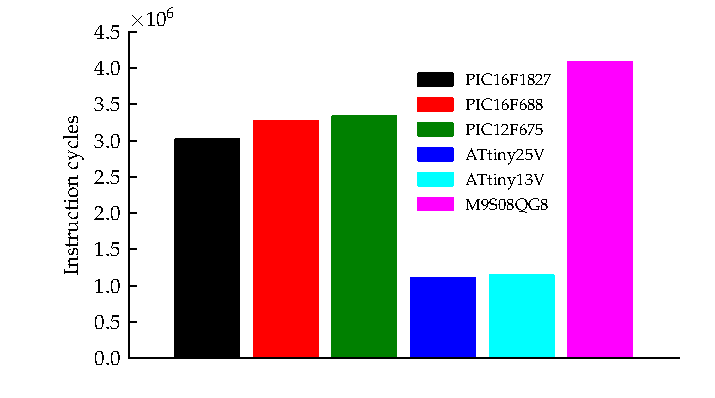
\includegraphics{content/pt1/03-EnergyRequirements/graphics/Graph_All_Clock_Benchmark}
    \end{centering}
    \protect\caption{\label{fig:GraphBar_All_Benchmark}MCU comparison of instructions
    taken to complete a benchmark.}
\end{figure}



\subsection{Non-volatile memory}

In order for a microprocessor to keep information about its current
state and recorded data in the event of power loss it must write to
non-volatile memory. Non-volatile memory is implemented as either
electrically erasable and programmable read only memory (EEPROM) or
Flash memory. Flash memory is similar to EEPROM with the exception
that it must be erased in large blocks, or pages, before it can be
written to. All of the tested MCUs have on-board EEPROM with the exception
of the MC9S08QG8 which has flash memory instead. Table \ref{tab:MCUfeaturecomparison}
shows the amount of non-volatile memory space available on each of
the chips. The energy consumption of each of the chips with EEPROM
memory during a 1-byte write operation (which also includes a 1-byte
erase operation) is shown in figure \ref{fig:Energy-consumed-EEPROM}.
There appears to be a glitch with the PIC12F675 with respect to it's
energy consumption. It's energy consumption was calculated as negative
with a Vdd below 4.7V, meaning that it consumed less current while
performing write operations than running through the same program
loop without performing writes. The measurement was repeated several
times and produced the same result but I did not further pursue the
cause. I have concluded that this is not representative of the MCU
and have disregarded EEPROM measurement data for this chip. In the
case of the MC9S08QG8, which has Flash memory instead of EEPROM, the
power consumption in the E + W case was calculated per erase/write
operation to be $1/512^{th}$ of the page erase energy consumption
added to the energy cost of a single write operation, where the W
case was the energy cost of a single write operation. In order for
the MC9S08QG8 to perform a write operation, the destination byte must
have already been pre-erased at an earlier point in time. This may
be useful for power harvesting since the energy expensive page erase
operation, which consumes an average of 3.02e-4 Joules, can be done
performed when available energy is plentiful.

\begin{figure}
\begin{centering}
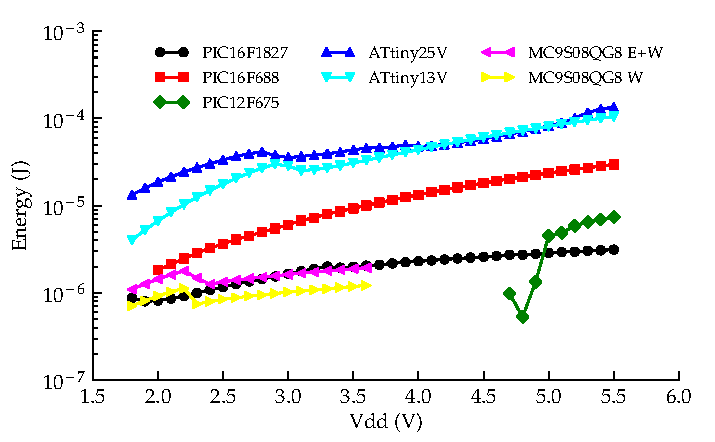
\includegraphics{content/pt1/03-EnergyRequirements/graphics/Graph_All_EEPROM_JPO}
\par\end{centering}

\protect\caption{Energy consumed by each MCU per non-volatile erase/write operation.\label{fig:Energy-consumed-EEPROM}}
\end{figure}



\subsection{Analog-to-digital conversions.}

To measure the flow of water the chosen MCU will likely either count
pulses record a voltage level from a flow meter. It is possible that
another mechanism such as ultrasonic flow measurement may be used
but for now only analog-to-digital (ADC) measurements will be measured.
For those unfamiliar with an ADC, it is simply a way of converting
a voltage (which is generally free to change) into a digital number
that a MCU can process and/or store. The power consumption per ADC
measurement for each of the tested MCUs is shown in figure \ref{fig:Energy-consumed-ADC}.

\begin{figure}
\begin{centering}
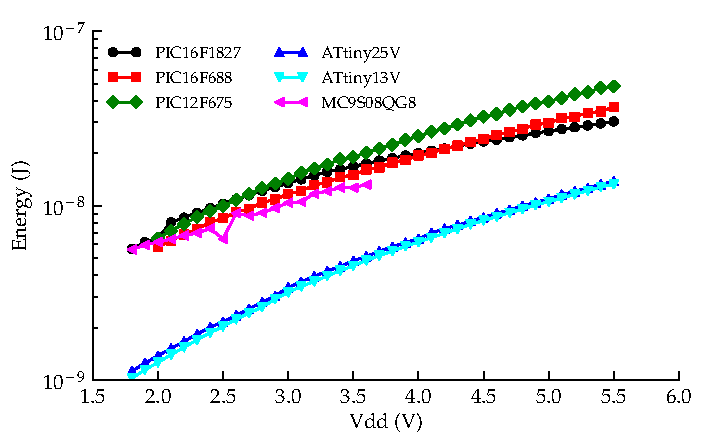
\includegraphics{content/pt1/03-EnergyRequirements/graphics/Graph_ALL_ADC_JPM}
\protect\caption{Energy consumed by each MCU per ADC measurement.\label{fig:Energy-consumed-ADC}}

\par\end{centering}

\end{figure}


\section{Wireless Transmission}
